The Commission for Energy Regulation (CER), the regulator for Ireland's electricity and natural gas sectors, conducted the Smart Metering Electricity Consumer Behavior Trial (hereafter, the ``trial'') between July 2009 and December 2010. As part of the Smart Metering Project initiated in 2007, the trial's purpose was to assess the impact of various TOU tariff structures, along with different Demand-Side Management (DSM) stimuli, on residential electricity consumption. The CER carefully recruited households to construct a representative sample of the national population. Opt-in to the trial was voluntary. Participants received balancing credits not to incur any extra costs than if they were on the regular electric tariff (i.e., the flat rate of 14.1 cents per kWh). Also, they received a thank-you payment of 25 cents after pre- and post-trial surveys. All credits were distributed outside the treatment period to avoid unintended effects on participants' electricity consumption.\footnote{While the first balancing credit was paid at the end of the base period (i.e., in December 2009), the participants received the second one at the immediate month after the treatment period (i.e., in January 2011). And the after-survey payments were credited to their bill with the balancing credits.}

The households who voluntarily opt-in to the experiment were randomly assigned to control and treatment groups.\footnote{The optimal sample size for the trial was determined to be 4,300 participants in the design phase. In the allocation phase, 5,028 households were assigned to the control and treatment groups to consider participant attrition. The published CER experiment data include electricity consumption data only for 4,225 households.} Baseline electricity consumption data were collected during the second half of 2009 (i.e., July to December 2009), while the treatment period was from January through December 2010. All treated households received two kinds of treatments simultaneously: 1) one of four TOU tariff structures and 2) one of four DSM stimuli, described in detail later. In other words, there were 16 distinct treatment subgroups. The CER provided the treated with a fridge magnet and stickers to facilitate accustoming them to the TOU pricing schemes.\footnote{The fridge magnet and stickers outlined the timebands during which different prices were applied. Moreover, they were tailored for each tariff group.} On the contrary, the households allocated to the control group remained on the normal flat tariff.

The four TOU tariff structures had different prices during each of the three rate periods in a day. The day in the treatment period was divided into three periods: 1) peak rate period from 5:00 p.m to 7:00 p.m., 2) day rate period from 8:00 a.m. to 5:00 p.m. and from 7:00 p.m. to 11:00 p.m., and 3) night rate period from 11:00 p.m. to 8:00 a.m. As illustrated in Figure \ref{Figure:Time-Of-Use-Pricing-Structures}, the order of magnitude in rate changes during the peak rate period is the opposite of that for the rest of the rate periods. The reason for designing the tariff structures in such a way is to enable participating households to face similar energy bills on average when maintaining their electricity consumption pattern, regardless of the rate structures to which they were assigned. 

The four DSM stimuli differed in the degree or the frequency of feedback on each household's electricity usage information. The control group received their bills in the same cycle (i.e., bi-monthly). On the contrary, all households assigned to the treatment group received a detailed energy usage statement combined with their bill, including their detailed weekly usage, average weekly costs, tips on reducing electricity use, and comparisons to peer households. The first stimulus subgroup received a bill with a detailed energy statement bi-monthly, while the second subgroup received the documents every month. An electricity monitor, which displays their usage against their pre-set daily budget, was also provided for the households allocated to the third DSM stimulus subgroup. The last stimulus subgroup received an Overall Load Reduction (OLR) incentive. Under the OLR incentive, the households that reached their 10\% reduction target over the eight-month period beginning May 2010 were rewarded with 20 Euros.\footnote{A household's reduction target in electricity consumption was set based on the participant's actual usage during the first four months of the treatment period. And the households in the last DSM stimulus subgroup were updated on their progress with each bi-monthly bill.}

\begin{figure}[!th]
%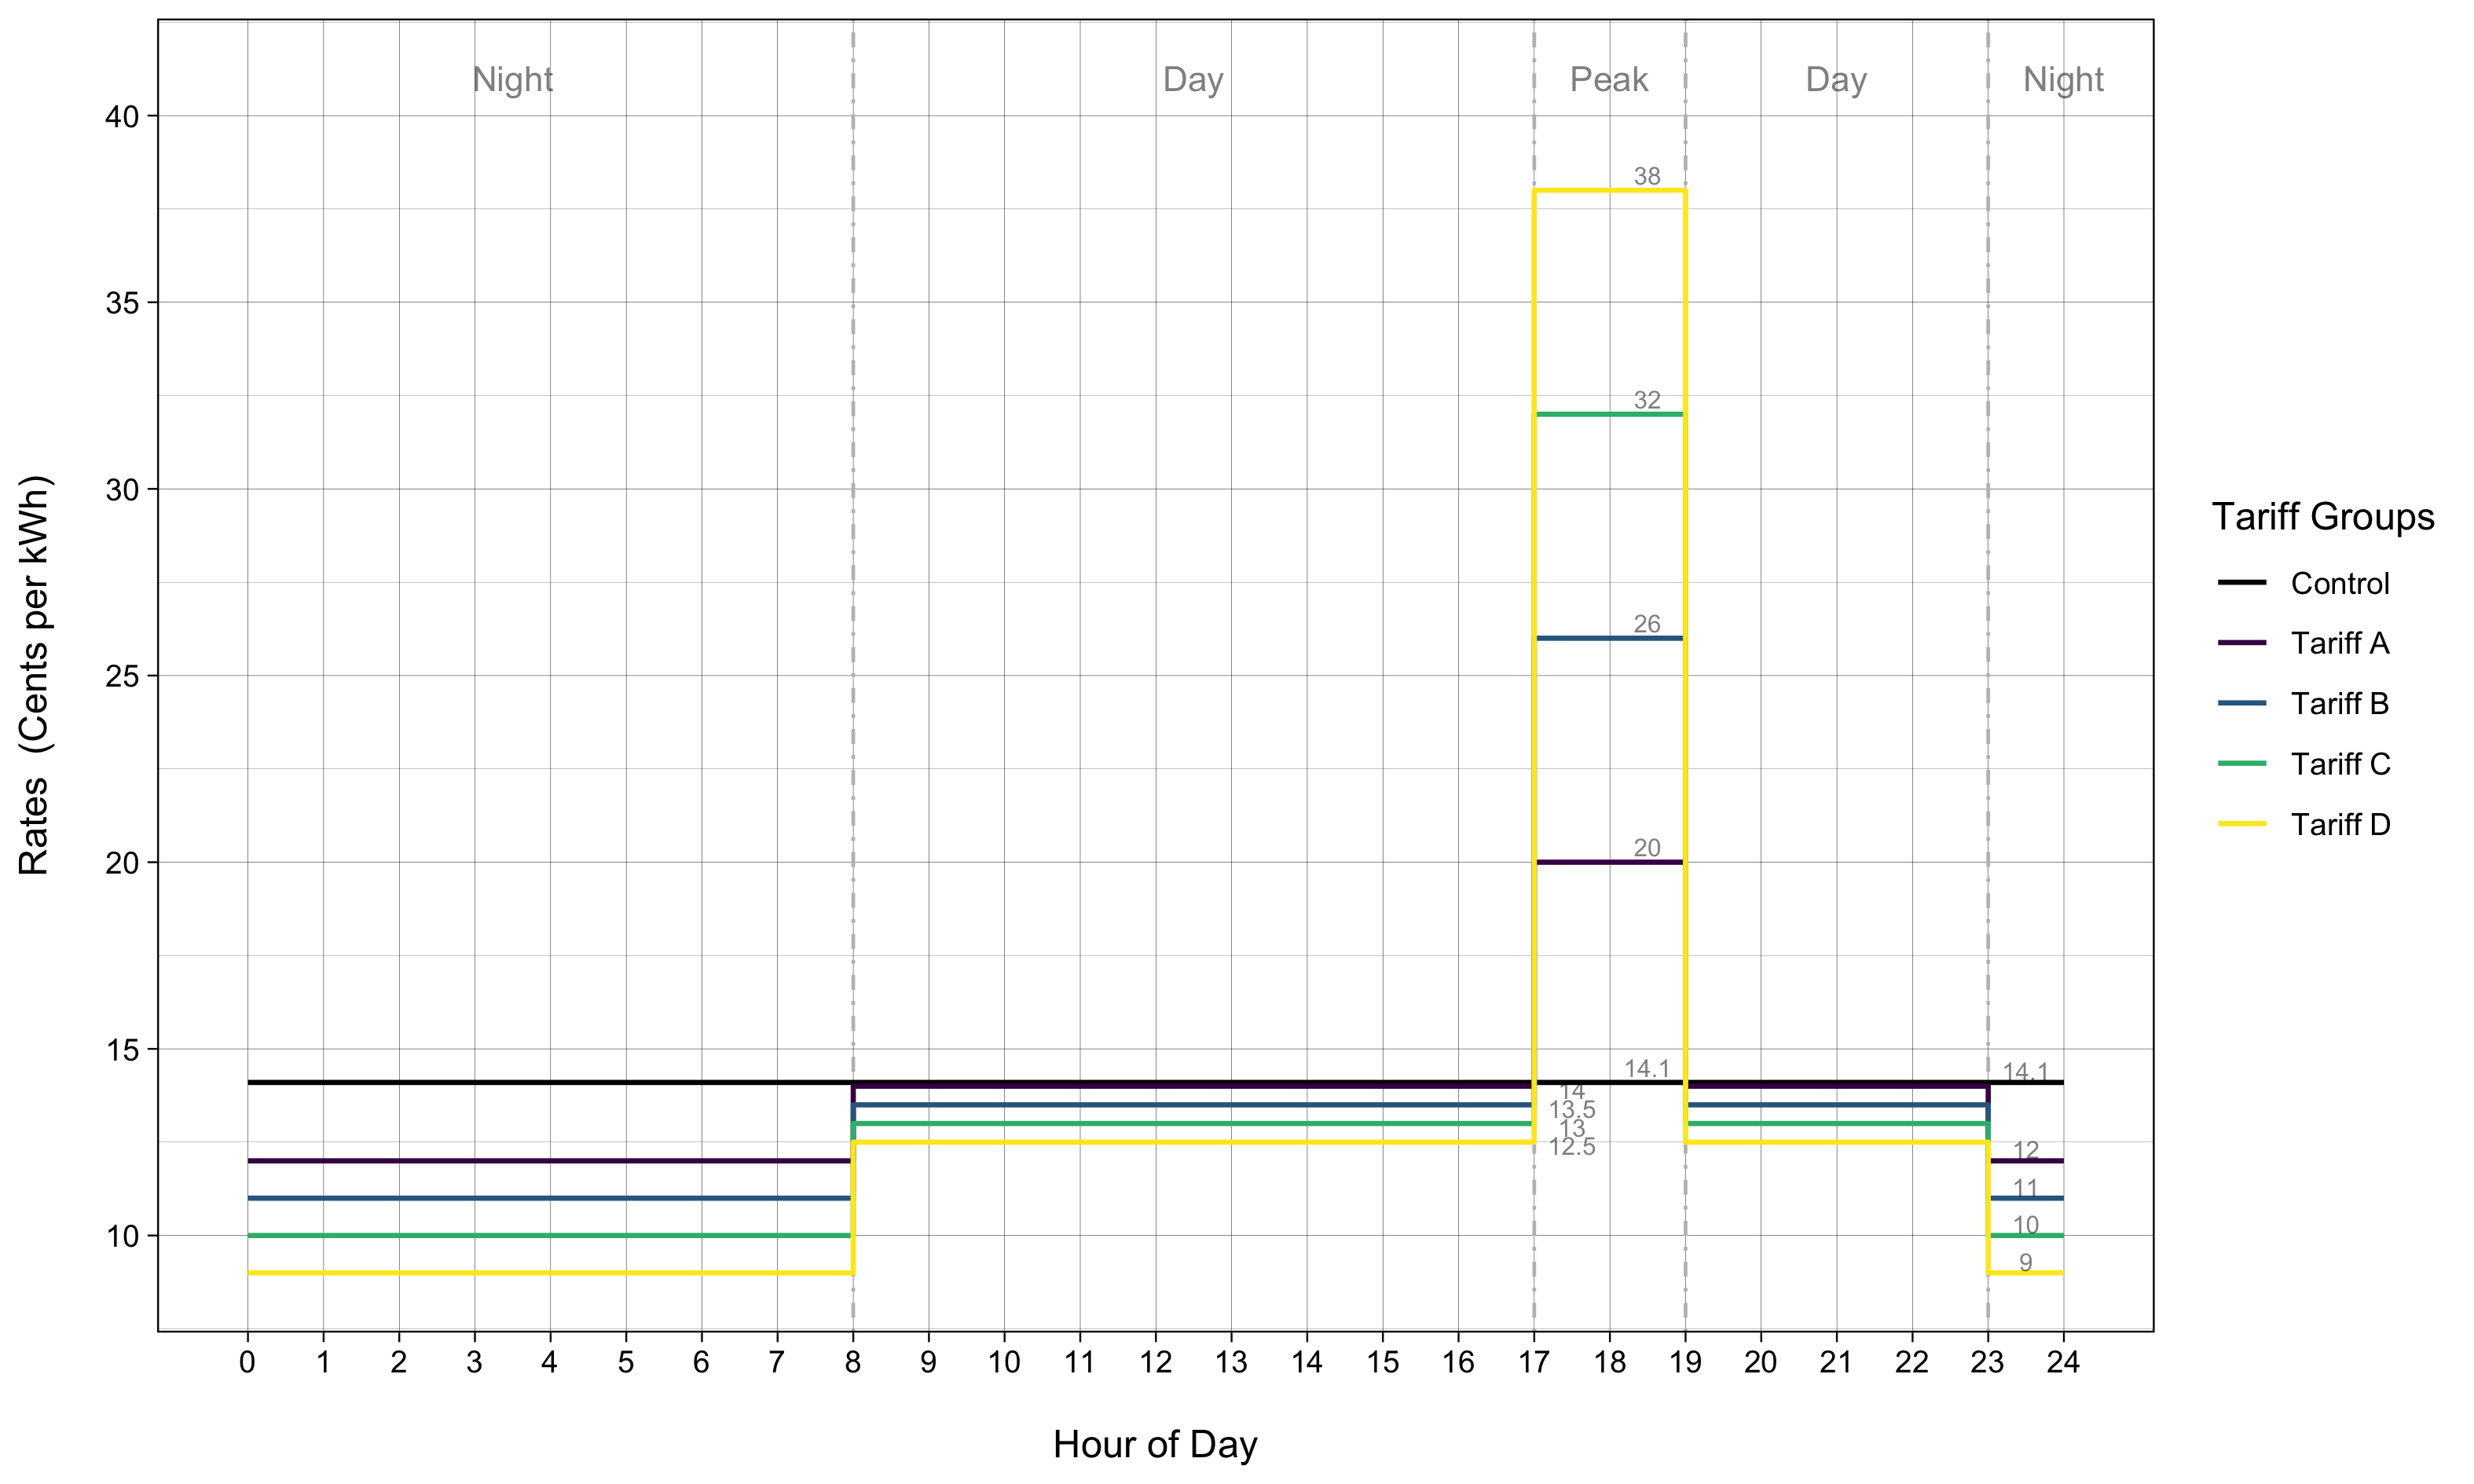
\includegraphics[scale = 0.095]{03_Chapter-2/00A_Figures/Figure_Time-of-Use-Tariff-Structures}
\caption{Time-Of-Use Pricing Structures}
\label{Figure:Time-Of-Use-Pricing-Structures}
\end{figure}
